\documentclass[11pt,a4paper]{article}
\usepackage[utf8]{inputenc}
\usepackage[T1]{fontenc}
\usepackage{mathptmx}
\usepackage[a4paper,margin=2.4cm]{geometry}
\usepackage{amsmath,amssymb}
\usepackage{graphicx,booktabs,float,xcolor,multirow,enumitem}
\usepackage{tikz}
\usetikzlibrary{positioning,arrows.meta,calc,decorations.pathreplacing}
\usepackage[font=small,labelfont=bf]{caption}
\usepackage[colorlinks=true,linkcolor=blue!50!black,citecolor=blue!50!black,urlcolor=blue!50!black]{hyperref}
\setlist{itemsep=2pt,topsep=3pt}
\setlength{\parskip}{3pt}
\newcommand{\NBN}{N_{\mathrm{BN}}}
\newcommand{\DVVS}{D_{\mathrm{VVS}}}

\title{\textbf{Retinal bottleneck in anatomically constrained CNNs}\\[2pt]
\large A reduced-scale reproduction of Lindsey et al.\ (ICLR 2019) on STL-10 and Imagenette}
\author{Alessandro Capialbi\\ Deep Learning, Prof.\ A.\ Asperti}
\date{October 2026}

\begin{document}
\maketitle

\begin{abstract}
\noindent Lindsey et al.\ (2019) train a convolutional network on object recognition, split into a ``retina'' and a ``ventral visual stream'', and show that two classical facts of visual neuroscience emerge from a single model: the retinal output has center-surround receptive fields while the first cortical layer has oriented ones, provided that the retinal output is a narrow bottleneck; and the depth of the cortex determines how linear and information-preserving the retina is. We reproduce their experiments at reduced scale on STL-10 and Imagenette (grayscale, $96\times96$, 3 seeds): 72 networks for the bottleneck sweep, 54 for a cortex-depth grid, and 18 networks in the paper's own setting (CIFAR-10) as a positive control. The accuracy claim (accuracy grows with bottleneck width and cortex depth) is reproduced. The retinal geometry is reproduced only partially: at the paper's headline configuration (one bottleneck channel, two cortical layers) the retinal orientation index is $1.47$ on Imagenette (paper: $1.56$) but $2.90$ on STL-10, the CIFAR-10 control gives $1.60$, and elsewhere in the sweep most retinal filters are oriented. Retinal linearity grows with cortex depth only at the tightest bottleneck, and the first cortical layer is more oriented than the retina at narrow bottlenecks. We document each difference from the original setup and report what we could and could not isolate.
\end{abstract}

\section{Introduction}
Why do retinal ganglion cells respond to local contrast while neurons in the primary visual cortex (V1) respond to oriented edges? Classical theories of efficient coding explain each geometry separately, but not why two consecutive stages should differ. Lindsey et al.\ \cite{lindsey2019} propose that the difference follows from a \emph{resource constraint}: the optic nerve carries the signal of roughly a hundred million photoreceptors through about one million fibres, so the retina is a dimensionality bottleneck. They model the visual system as a deep CNN trained for object recognition, vary the width of the retinal output and the depth of the cortex, and look at the receptive fields (RFs) that emerge.

The assignment of this project is a \emph{reduced-scale reproduction} of that paper on two datasets chosen by the instructor, STL-10 and Imagenette at $96\times96$, with the ablations of bottleneck width, retina depth and cortex depth, and three seeds per configuration. The aim is not to match the numbers of the paper but to measure carefully what survives the change of setting and to say why, or why we cannot say. The report is organised as follows: Section~\ref{sec:bg} gives the neuroscience needed to read the paper; Section~\ref{sec:paper} summarises its model and claims; Section~\ref{sec:setup} describes our setup and every difference from the original; Section~\ref{sec:res} reports the results, including a positive control run in the original setting; Sections~\ref{sec:disc}--\ref{sec:concl} discuss, list the limitations and conclude.

\section{Background: the early visual system}\label{sec:bg}
\paragraph{From the eye to the cortex.} Light is transduced by photoreceptors (rods and cones). Their signal passes through bipolar cells to the \emph{retinal ganglion cells}, whose axons form the optic nerve. In humans there are of the order of $10^8$ photoreceptors and $10^6$ ganglion cells, a compression of about two orders of magnitude, so the optic nerve is a stringent bottleneck. The signal is relayed by the thalamus (lateral geniculate nucleus, LGN) to the primary visual cortex V1 and then along the \emph{ventral stream} (V2, V4, inferotemporal cortex), which supports object recognition.

\paragraph{Receptive fields.} The receptive field (RF) of a neuron is the part of the visual scene, and the kind of pattern, that drives it. Two geometries matter here (Fig.~\ref{fig:model}b).
\begin{itemize}
\item \emph{Center-surround} RFs of retinal ganglion cells (and LGN): a small excitatory center surrounded by an inhibitory ring, or the opposite (ON and OFF cells). They respond to local contrast and not to uniform illumination, and act as a decorrelating (whitening) filter.
\item \emph{Oriented} RFs of V1 simple cells: elongated patches responding to an edge of a given orientation and position, well described by Gabor functions. Hubel and Wiesel \cite{hubel1962} hypothesised that they are built by pooling center-surround inputs aligned along the edge; complex cells then pool simple cells and add position invariance.
\end{itemize}

\paragraph{The open question.} Efficient-coding theories reproduce center-surround RFs (decorrelation of natural images under noise \cite{atick1990}) and oriented RFs (sparse coding \cite{olshausen1996}), but with different objectives and constraints for the two stages. Moreover, retinas differ across species: in primates the most common ganglion cell type is close to a linear pixel encoder (midget cells), while in the mouse the most common type is a nonlinear feature detector \cite{roska2014}, and the frog retina detects behaviourally relevant stimuli. A single account should explain both the retina--V1 difference and the diversity across species.

\section{The reference paper}\label{sec:paper}
\paragraph{Model.} The paper trains a CNN on grayscale CIFAR-10 \cite{krizhevsky2009} (Fig.~\ref{fig:model}a). A \emph{retina-net} of two convolutions (32 channels, then $\NBN$ channels, the retinal output) feeds a \emph{ventral-visual-system net} (VVS-net) of $\DVVS$ convolutions with 32 channels followed by two dense layers (1024 and 10 units). All convolutions are $9\times9$, stride 1, with ReLU and no batch normalisation; training uses RMSProp for 20 epochs, batch size 32, Glorot-uniform initialisation \cite{glorot2010}, ten random initialisations per architecture (Keras/TensorFlow). The RF of a channel is estimated as the gradient of its activation at the image centre with respect to a blank image, equivalent to a spike-triggered average for a small perturbative stimulus.

\begin{figure}[t]
\centering
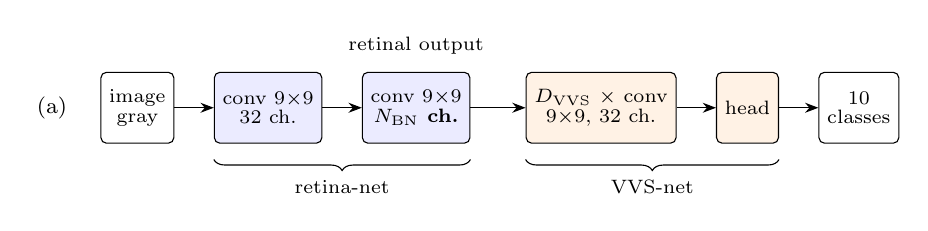
\begin{tikzpicture}[node distance=5mm, box/.style={draw, rounded corners=2pt, minimum height=9mm, align=center, font=\scriptsize, inner sep=3pt}]
\node[box] (img) {image\\[-1pt]gray};
\node[box, right=of img, fill=blue!8] (r1) {conv $9{\times}9$\\[-1pt]32 ch.};
\node[box, right=of r1, fill=blue!8] (r2) {conv $9{\times}9$\\[-1pt]\textbf{$\NBN$ ch.}};
\node[box, right=7mm of r2, fill=orange!10] (v) {$\DVVS$ $\times$ conv\\[-1pt]$9{\times}9$, 32 ch.};
\node[box, right=of v, fill=orange!10] (h) {head};
\node[box, right=of h] (o) {10\\[-1pt]classes};
\draw[-{Stealth}] (img)--(r1); \draw[-{Stealth}] (r1)--(r2); \draw[-{Stealth}] (r2)--(v); \draw[-{Stealth}] (v)--(h); \draw[-{Stealth}] (h)--(o);
\draw[decorate, decoration={brace, amplitude=4pt, mirror}] ($(r1.south west)+(0,-2mm)$) -- node[below=4pt, font=\scriptsize]{retina-net} ($(r2.south east)+(0,-2mm)$);
\draw[decorate, decoration={brace, amplitude=4pt, mirror}] ($(v.south west)+(0,-2mm)$) -- node[below=4pt, font=\scriptsize]{VVS-net} ($(h.south east)+(0,-2mm)$);
\node[font=\scriptsize, above=1mm of r2] {retinal output};
\node[font=\footnotesize, left=2mm of img, xshift=-1mm] {(a)};
\end{tikzpicture}\\[6pt]
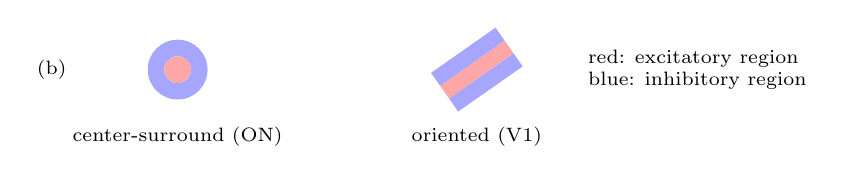
\begin{tikzpicture}[font=\scriptsize]
\node at (0,0) {(b)};
\begin{scope}[shift={(1.6,0)}]
 \fill[blue!35] (0,0) circle (0.38); \fill[white] (0,0) circle (0.17); \fill[red!35] (0,0) circle (0.17);
 \node[below=6mm] at (0,0) {center-surround (ON)};
\end{scope}
\begin{scope}[shift={(5.4,0)}]
 \begin{scope}[rotate=35]
 \fill[red!35] (-0.5,-0.1) rectangle (0.5,0.1); \fill[blue!35] (-0.5,0.1) rectangle (0.5,0.3); \fill[blue!35] (-0.5,-0.3) rectangle (0.5,-0.1);
 \end{scope}
 \node[below=6mm] at (0,0) {oriented (V1)};
\end{scope}
\node at (8.2,0) [align=left] {red: excitatory region\\blue: inhibitory region};
\end{tikzpicture}
\caption{(a) The architecture of the paper and of this project: a retina-net whose output is a bottleneck of $\NBN$ channels, followed by a cortex of $\DVVS$ convolutions and a classifier head. (b) The two receptive-field geometries of the early visual system.}\label{fig:model}
\end{figure}

\paragraph{Claims.} (i) \emph{A bottleneck at the retinal output} ($\NBN=4,2,1$) \emph{yields center-surround retinal RFs and oriented RFs in the first cortical layer}; with $\NBN=32$ the retinal RFs are oriented. The RF geometry does not depend qualitatively on $\DVVS$ (shown for $\DVVS=2$), except for $\DVVS=0$. (ii) \emph{The cortex depth sets the linearity of the retina:} with a deeper cortex the retinal response is more linear and keeps more information about the image but separates the classes less; with a shallow cortex the retina is nonlinear and extracts features. (iii) \emph{The accuracy increases with the bottleneck width and with the cortex depth} (their Fig.~1D).

\paragraph{Measures.} The \emph{orientation selectivity index} (OSI) is computed from the responses of an RF to rectangular bars of all widths, orientations and positions: the ratio between the strongest response at the preferred orientation and the strongest response at the orthogonal one. It is $\approx1$ for isotropic RFs and larger for oriented ones. The paper reports $1.56\pm0.22$ for the retinal output, $3.05\pm0.30$ for the first cortical layer, and $1.97\pm0.08$ for random-noise RFs. \emph{Linearity} is the Pearson correlation between the true response of a retinal unit and its ridge-regression prediction from the image; \emph{information} is the variance explained when the image is linearly reconstructed from the retinal output.

\section{Our reproduction: setup and differences}\label{sec:setup}
\subsection{Hypotheses of the assignment}
The assignment is phrased as three hypotheses: (H1) a narrow bottleneck with a deep cortex makes the retina learn center-surround filters; (H2) a wide bottleneck or a shallow cortex makes the retina learn oriented filters; (H3) the accuracy degrades little as the bottleneck narrows, until a minimum width. After reading the paper in full we note that H1 and H2 are stricter than claims (i) and (ii): the paper does not tie center-surround RFs to a deep cortex, nor oriented retinal RFs to a shallow one, and its cortex-depth effect is on the \emph{linearity} of the retina. We therefore test both the hypotheses as written and the paper's own claims.

\subsection{Data}
\begin{table}[b]
\centering\small
\begin{tabular}{p{1.9cm}p{2.5cm}p{2.5cm}p{4.2cm}p{3.0cm}}
\toprule
 & Resolution & Classes & Labelled train / test & Role here\\
\midrule
CIFAR-10 & $32{\times}32$ colour & 10 & 50\,000 / 10\,000 & paper's data; positive control\\
STL-10 & $96{\times}96$ colour & 10 & 5\,000 / 8\,000 (+100\,000 unlabelled, unused) & main dataset\\
Imagenette & up to $160$ px & 10 easy ImageNet classes & 9\,469 / 3\,925 & main dataset\\
\bottomrule
\end{tabular}
\caption{Datasets. STL-10 \cite{coates2011} is a subset of ImageNet with few labels per class; Imagenette is a ten-class ImageNet subset by fast.ai. A part of the training set (10\%) is held out for validation, so the networks are trained on about 4\,500 (STL-10) and 8\,500 (Imagenette) images, against 45\,000 for CIFAR-10.}\label{tab:data}
\end{table}
STL-10 and Imagenette are decoded once (resize to $96$, centre crop, grayscale) and kept as 8-bit tensors on the GPU. The test sets are the official STL-10 \texttt{test} split and the Imagenette \texttt{val} split. CIFAR-10 is not simply ``easier'': it has far more labels per class (5\,000 against 500 for STL-10) but a much lower resolution. The two properties that matter for the mechanism studied here are the resolution, relative to the $9{\times}9$ kernels, and the amount of training data.

\subsection{Architecture, training and differences from the paper}
Our network follows Fig.~\ref{fig:model}a with $\NBN\in\{1,2,4,8,16,32\}$, retina depth 1 or 2 (the last retina layer has $\NBN$ channels) and $\DVVS\in\{1,2,3,4\}$. Table~\ref{tab:diff} lists every difference from the original setup.
\begin{table}[t]
\centering\small
\begin{tabular}{p{2.6cm}p{5.4cm}p{6.6cm}}
\toprule
 & Paper & This project\\
\midrule
Data & grayscale CIFAR-10, $32{\times}32$, 50\,000 images & grayscale STL-10 / Imagenette, $96{\times}96$, 4\,500 / 8\,500 images (assignment)\\
Cortex head & flatten, dense 1024, dense 10 & $2{\times}2$ max-pool after every cortical conv, global average pool, linear layer (a flatten + dense 1024 at $96{\times}96$ would have hundreds of millions of weights)\\
Cortex depth & $\DVVS=0$--4 & 1--4; $\DVVS=0$ not run (no meaningful head)\\
Optimiser & RMSProp, 20 epochs, batch 32, Glorot-uniform & the same (RMSProp $\rho=0.9$, $\epsilon=10^{-7}$, lr $10^{-3}$); PyTorch\\
Not stated in the paper & input scaling, augmentation, checkpoint & input centred as $(x-0.5)/0.25$ inside the model; random horizontal flip; checkpoint with best validation accuracy\\
Collapsed runs & not discussed & a run whose best validation accuracy is below 0.2 is retrained once with lr/3; both kept\\
RF probe & gradient at a blank image & gradient averaged over 256 natural images (a flat image leaves 77\% of our retinal channels silent)\\
Seeds & 10 & 3\\
Extra analyses & separability, untied retina, LGN, simple/complex cells, normalisation & not reproduced\\
\bottomrule
\end{tabular}
\caption{Differences between the original setup and ours.}\label{tab:diff}
\end{table}

\subsection{Receptive-field analysis}
The RF of each retinal channel is the gradient of its activation at the image centre with respect to the pixels, averaged over 256 natural images; the input is centred exactly as in the forward pass of the network. The OSI uses the paper's definition. In addition, every RF is fitted with an isotropic difference of Gaussians (DoG) and with a Gabor function, and labelled \emph{center-surround} (OSI $<2$ and a DoG fit with $R^2\ge0.5$ not worse than the Gabor by more than $0.05$), \emph{oriented} (OSI $\ge2$, Gabor $R^2\ge0.5$ and better than the DoG), \emph{dead} (zero gradient) or \emph{other}. The thresholds were fixed on synthetic filters before looking at the learned ones (the classifier recovers the true class of 40/40 synthetic filters per class under 10\% noise). Because the labels depend on thresholds and fits, we also report the OSI itself, which is threshold free.

\subsection{Experiments}
\begin{itemize}
\item \textbf{Sweep (72 networks).} Two datasets $\times$ 12 configurations $\times$ 3 seeds: $\NBN\in\{1,\dots,32\}$ at retina depth 2 and cortex depth 2, plus $\NBN\in\{2,16\}$ with retina depth 1 or cortex depth 4. 3 of 72 runs collapsed and were retrained.
\item \textbf{Cortex-depth grid (54 networks).} $\NBN\in\{1,4,32\}$ at $\DVVS\in\{1,3,4\}$ (depth 2 comes from the sweep); 9 runs collapsed at the first attempt, 7 of them at $\NBN=1$.
\item \textbf{Linearity, information and first cortical layer} on all 126 networks, without new training.
\item \textbf{Positive control (18 networks).} The architecture of the paper, with flatten and dense layers and no pooling, on grayscale CIFAR-10 at $32{\times}32$ with our training recipe: $\NBN\in\{1,4,32\}$, $\DVVS\in\{2,4\}$, 3 seeds. The prediction and its decision rule were written before the runs.
\item \textbf{Recipe check (4 networks).} CIFAR-10, $\NBN\in\{4,32\}$, seed 0, to see whether our unstated choices (input centring, flip, checkpoint) matter.
\end{itemize}

\section{Results}\label{sec:res}
\subsection{Accuracy (claim iii)}
Test accuracy increases with the cortex depth in all six dataset--bottleneck cells (Fig.~\ref{fig:acc}, Table~\ref{tab:acc}): at $\NBN=1$ from $0.31$ to $0.56$ on STL-10 and from $0.42$ to $0.68$ on Imagenette between depth 1 and 4. At depth 2 it increases with the width, from $0.417$ to $0.519$ (STL-10) and from $0.553$ to $0.663$ (Imagenette) between 1 and 32 channels, with small non-monotonic steps. We do not observe a knee: going from 32 to 1 channel costs about ten points on both datasets, and no narrower bottleneck comes within one point of the widest one. Both parts of claim (iii) are reproduced; H3 as formulated (little loss until a minimum width) is not. Absolute accuracies are low (0.31--0.69) because of the small training sets.
\begin{figure}[t]\centering
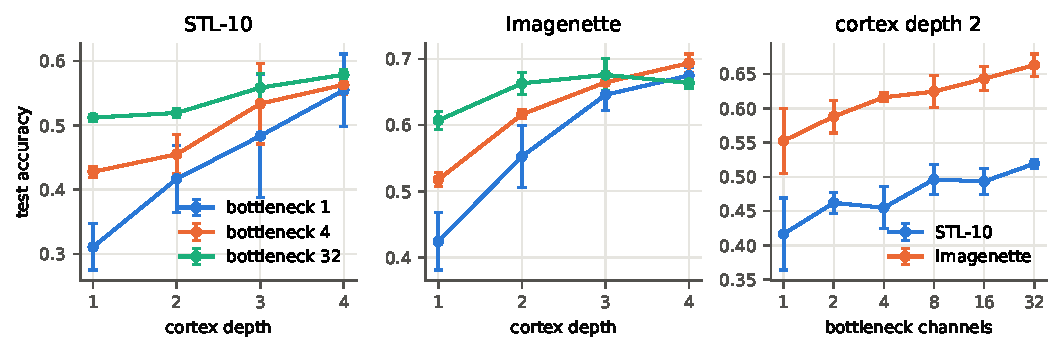
\includegraphics[width=\textwidth]{figs/fig_accuracy.pdf}
\caption{Test accuracy (mean $\pm$ s.d.\ over 3 seeds) against cortex depth for three bottlenecks (left, centre) and against bottleneck width at cortex depth 2 (right).}\label{fig:acc}
\end{figure}
\begin{table}[t]\centering\small
\begin{tabular}{lrcccc}
\toprule
Dataset & $N_{BN}$ & depth 1 & depth 2 & depth 3 & depth 4 \\
\midrule
STL-10 & 1 & 0.311 $\pm$ 0.036 & 0.417 $\pm$ 0.053 & 0.483 $\pm$ 0.096 & 0.555 $\pm$ 0.056 \\
STL-10 & 4 & 0.428 $\pm$ 0.008 & 0.455 $\pm$ 0.030 & 0.534 $\pm$ 0.063 & 0.563 $\pm$ 0.015 \\
STL-10 & 32 & 0.512 $\pm$ 0.005 & 0.519 $\pm$ 0.007 & 0.559 $\pm$ 0.022 & 0.579 $\pm$ 0.007 \\
Imagenette & 1 & 0.424 $\pm$ 0.043 & 0.553 $\pm$ 0.047 & 0.646 $\pm$ 0.024 & 0.675 $\pm$ 0.013 \\
Imagenette & 4 & 0.518 $\pm$ 0.010 & 0.616 $\pm$ 0.007 & 0.665 $\pm$ 0.016 & 0.694 $\pm$ 0.014 \\
Imagenette & 32 & 0.607 $\pm$ 0.014 & 0.663 $\pm$ 0.016 & 0.676 $\pm$ 0.024 & 0.664 $\pm$ 0.009 \\
\bottomrule
\end{tabular}

\caption{Test accuracy (mean $\pm$ s.d.\ over 3 seeds) by cortex depth. Part of the deep $\NBN=1$ runs are reruns with lr/3 after a collapse.}\label{tab:acc}
\end{table}

\subsection{Retinal receptive fields (claim i)}
\paragraph{Geometry.} Of the 702 retinal channels of the sweep, 22 (3.1\%) are labelled center-surround, 270 oriented, 316 other and 94 dead (13\%) (Table~\ref{tab:labels}, Fig.~\ref{fig:labels}). Even the unlabelled quantity points the same way: the median OSI of the 608 live channels is $2.5$, against $1.56$ in the paper, and 37\% have OSI $<2$. The label is conservative (the 22 center-surround channels have DoG and Gabor $R^2$ within $0.10$ of each other, and isotropic filters with a poor DoG fit are labelled ``other'', median OSI 1.8), so we rely on the OSI as well. Fig.~\ref{fig:rfs} shows examples.

\paragraph{The paper's headline configuration} ($\NBN=1$, cortex depth 2) gives a live retinal channel per network. On Imagenette their OSI is $1.22$, $1.51$ and $1.69$ (mean $1.47$, close to the $1.56$ of the paper; all three below 2) but on STL-10 it is $1.84$, $3.23$ and $3.62$ (mean $2.90$). Pooling the narrow bottlenecks (1--2 channels, cortex depth 2), 6 of 9 live channels have OSI $<2$ on Imagenette against 32 of 125 at 16--32 channels; on STL-10 the figures are 2 of 9 against 37 of 111, i.e.\ no effect (Fig.~\ref{fig:osi}). With at most 9 channels at the narrow end, the effect is therefore dataset dependent and suggestive only.
\begin{table}[t]\centering\small
\begin{tabular}{lrrrrrrrr}
\toprule
Dataset & $N_{BN}$ & Channels & C-S & Orient. & Other & Dead & Median OSI & OSI$<$2 \\
\midrule
STL-10 & 1 & 3 & 0 & 2 & 1 & 0 & 3.23 & 1/3 \\
STL-10 & 2 & 6 & 1 & 5 & 0 & 0 & 2.33 & 1/6 \\
STL-10 & 4 & 12 & 0 & 6 & 5 & 1 & 2.71 & 5/11 \\
STL-10 & 8 & 24 & 0 & 15 & 4 & 5 & 3.26 & 2/19 \\
STL-10 & 16 & 48 & 1 & 22 & 15 & 10 & 2.63 & 14/38 \\
STL-10 & 32 & 96 & 2 & 49 & 22 & 23 & 2.85 & 23/73 \\
Imagenette & 1 & 3 & 1 & 0 & 2 & 0 & 1.51 & 3/3 \\
Imagenette & 2 & 6 & 3 & 3 & 0 & 0 & 2.33 & 3/6 \\
Imagenette & 4 & 12 & 0 & 10 & 1 & 1 & 2.87 & 0/11 \\
Imagenette & 8 & 24 & 1 & 13 & 7 & 3 & 3.51 & 6/21 \\
Imagenette & 16 & 48 & 2 & 28 & 13 & 5 & 2.86 & 14/43 \\
Imagenette & 32 & 96 & 2 & 54 & 26 & 14 & 3.56 & 18/82 \\
\bottomrule
\end{tabular}

\caption{Labels of the retinal channels of the sweep (retina depth 2, cortex depth 2; C-S = center-surround), median OSI of the live channels and number of live channels with OSI $<2$.}\label{tab:labels}
\end{table}
\begin{figure}[t]\centering
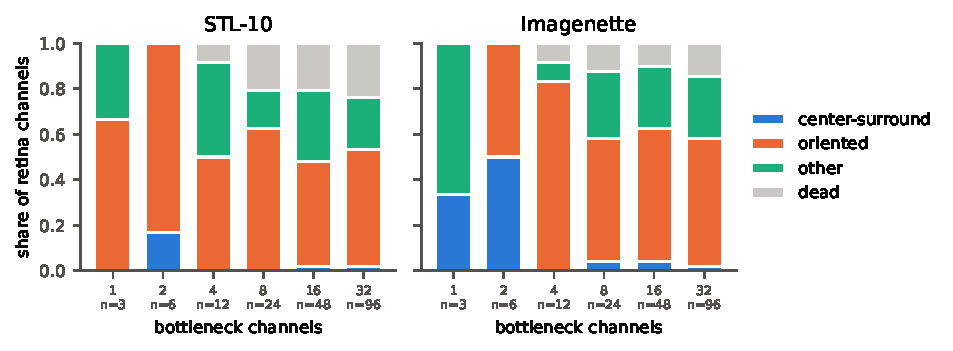
\includegraphics[width=0.92\textwidth]{figs/fig_labels.pdf}
\caption{Composition of the retinal channels by label for each bottleneck (retina depth 2, cortex depth 2). $n$ is the number of retinal channels (3 seeds $\times$ bottleneck width).}\label{fig:labels}
\end{figure}
\begin{figure}[t]\centering
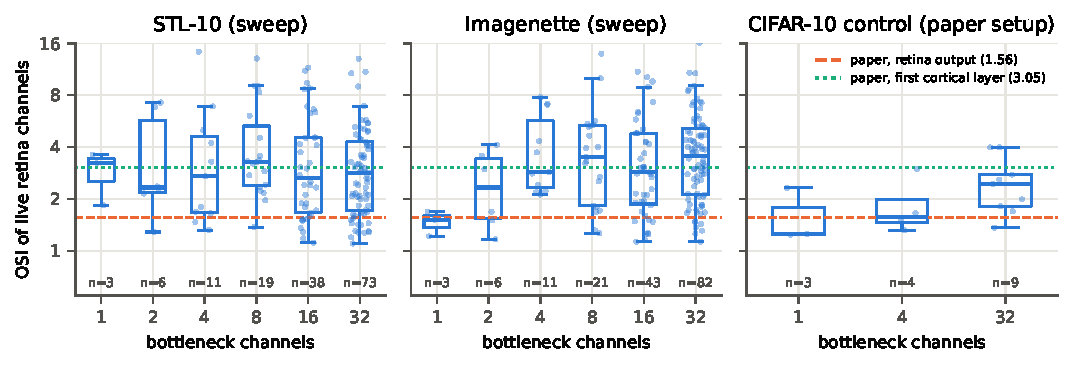
\includegraphics[width=\textwidth]{figs/fig_osi.pdf}
\caption{OSI of the live retinal channels at cortex depth 2: sweep on STL-10 and Imagenette, and CIFAR-10 control (bottleneck widths 1, 4, 32). Dashed: paper's retinal OSI; dotted: paper's first cortical layer.}\label{fig:osi}
\end{figure}
\begin{figure}[t]\centering
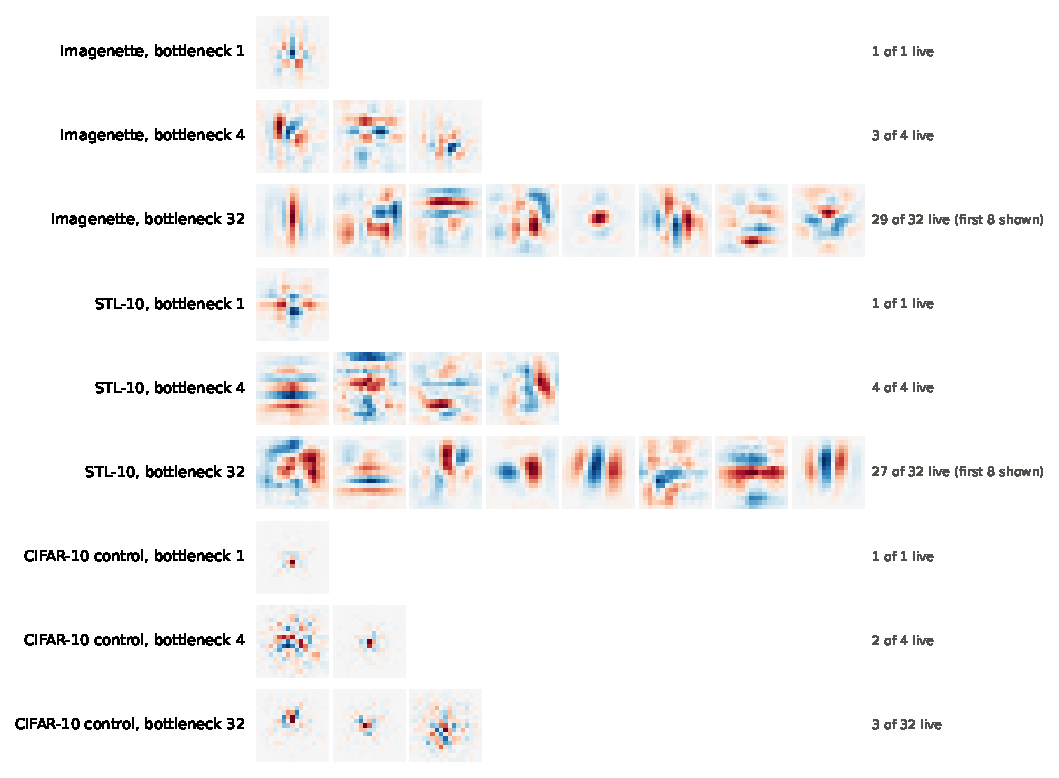
\includegraphics[width=0.95\textwidth]{figs/fig_rfs.pdf}
\caption{Retinal receptive fields (seed 0, cortex depth 2; red positive, blue negative, each scaled to its own maximum). Top: Imagenette and STL-10 sweep; bottom: CIFAR-10 control. At the narrowest bottleneck the single channel is compact and isotropic on Imagenette and on CIFAR-10; with 32 channels most filters are elongated.}\label{fig:rfs}
\end{figure}

\paragraph{H1 and H2 as written.} In the configuration of H1 ($\NBN=2$, cortex depth 4) only 1 of 6 channels is center-surround on each dataset, 3 of 6 are oriented and the median OSI is $2.7$ (STL-10) and $2.0$ (Imagenette): H1 is not reproduced. For H2, bottleneck 32 has 49/96 and 54/96 oriented channels, but narrow bottlenecks are not less oriented on STL-10 (7 of 9 channels at 1--2 channels) and less so on Imagenette (3 of 9). With the bottleneck fixed, cortex depth 2 has more oriented channels than cortex depth 4 in three of four comparisons and a tie in the fourth (e.g.\ $\NBN=16$: 22/48 against 14/48 on STL-10, 28/48 against 16/48 on Imagenette), consistent with H2 as worded; this is not a claim of the paper, which reports no dependence of the geometry on the depth. With retina depth 1 most filters are ``other'' and the $9{\times}9$ RF is too small for the fits to be reliable.

\subsection{First cortical layer (claim i, second half)}
The first cortical layer has all its 32 channels alive and median OSI between $2.4$ and $5.3$, around the $3.05$ of the paper (Fig.~\ref{fig:layer1}). It is more oriented than the retinal output at narrow bottlenecks (1--4 channels) in 4 of 6 cells ($\NBN=1$: $3.3$ against $1.5$ on Imagenette, $5.3$ against $2.9$ on STL-10), while at wide bottlenecks the retina is itself oriented and there is no difference (4 of 12 cells in total). The retina-to-cortex step from isotropic to oriented RFs is therefore visible at the tightest bottleneck, in agreement with the paper.
\begin{figure}[t]\centering
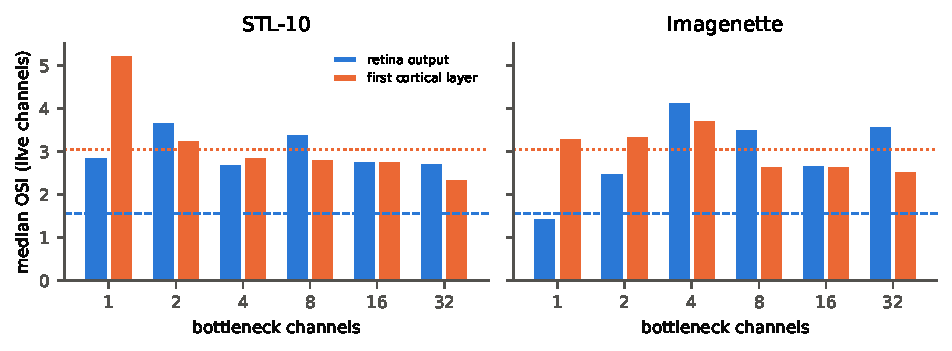
\includegraphics[width=0.92\textwidth]{figs/fig_layer1.pdf}
\caption{Median OSI of the live channels of the retinal output and of the first cortical layer (cortex depth 2). Dashed: paper's retina (1.56); dotted: paper's first cortical layer (3.05).}\label{fig:layer1}
\end{figure}

\subsection{Linearity and information (claim ii)}
Linearity of the retinal response (Fig.~\ref{fig:lin}, top) \emph{decreases with the bottleneck width} at depth 2 (Imagenette $0.73$ at 1 channel to $0.42$ at 32; STL-10 $0.62$ to $0.39$), as in the paper. It \emph{increases with the cortex depth only at $\NBN=1$}: from $0.52$ to $0.76$ (STL-10) and from $0.65$ to $0.76$ (Imagenette) between depth 1 and 4, which is the case the paper highlights (about 0.9 of the variance explained at one channel with the deepest cortex). At $\NBN=4$ and 32 the trend is flat or non-monotonic with a maximum at depth 2 (the paper reports a maximum at depth 1 without bottleneck). A deeper cortex also leaves fewer live retinal channels at width 32 (STL-10: 27 at depth 1, 12.7 at depth 4), so these means are over a shrinking set. The information kept by the retina (local reconstruction of the centre pixel from a $9{\times}9$ window of retinal output; Fig.~\ref{fig:lin}, bottom) increases with depth in 4 of 6 cells (e.g.\ STL-10 at one channel from $0.08$ to $0.36$) and is flat in the other two; it grows with the width, as it must. Claim (ii) is reproduced in the tightest-bottleneck case, which is also the one where the retina has a single channel and where the paper finds the strongest effect.
\begin{figure}[t]\centering
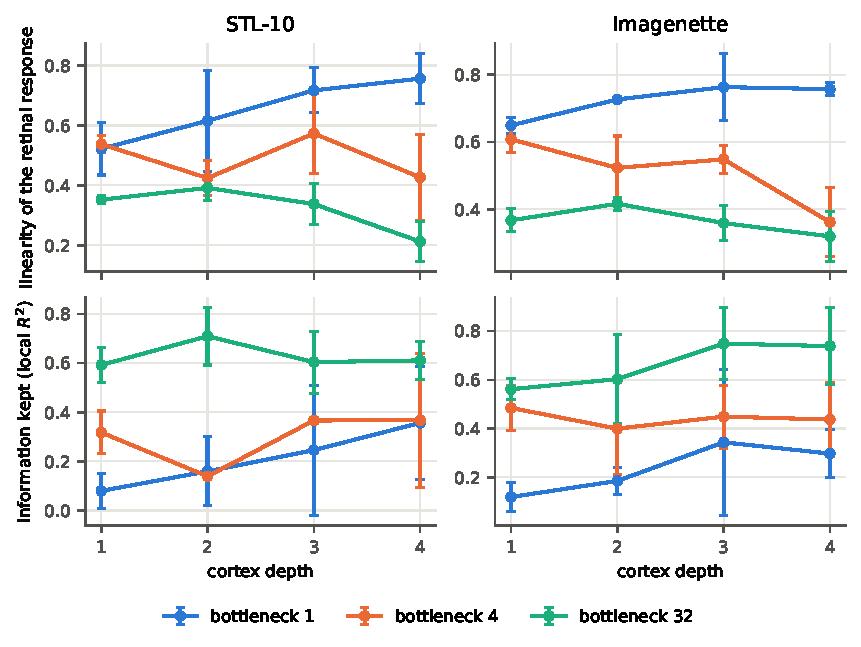
\includegraphics[width=0.78\textwidth]{figs/fig_linearity.pdf}
\caption{Linearity of the retinal response and local information kept by the retina against cortex depth (mean $\pm$ s.d.\ over 3 seeds, live channels only).}\label{fig:lin}
\end{figure}

\subsection{Positive control in the paper's own setting}
To separate the effect of our setup from the effect of our analysis, we trained the architecture of the paper on grayscale CIFAR-10 (Table~\ref{tab:ctrl}). The recipe is fragile in our hands: accuracy is $0.56$--$0.67$ (similar to the range of $0.5$--$0.7$ on the axis of their Fig.~1D), 6 of 18 runs collapsed at the first attempt (5 at one channel), and 67\% of the retinal channels are dead (149 of 222) against 13\% in the sweep.
\begin{table}[t]\centering\small
\begin{tabular}{rrcrrrrr}
\toprule
$N_{BN}$ & Depth & Test acc. & Collapsed & Live/ch. & C-S & Median OSI & OSI$<$2 \\
\midrule
1 & 2 & 0.672 $\pm$ 0.004 & 3 & 3/3 & 1 & 1.25 & 2/3 \\
1 & 4 & 0.652 $\pm$ 0.079 & 2 & 3/3 & 0 & 2.31 & 1/3 \\
4 & 2 & 0.605 $\pm$ 0.024 & 0 & 4/12 & 2 & 1.58 & 3/4 \\
4 & 4 & 0.555 $\pm$ 0.022 & 0 & 4/12 & 2 & 1.85 & 2/4 \\
32 & 2 & 0.594 $\pm$ 0.021 & 0 & 9/96 & 1 & 2.44 & 4/9 \\
32 & 4 & 0.573 $\pm$ 0.092 & 1 & 50/96 & 1 & 2.55 & 18/50 \\
\bottomrule
\end{tabular}

\caption{CIFAR-10 control (paper's architecture, natural-image probe): collapsed first attempts, live channels out of the channels of the 3 seeds, center-surround labels, and OSI.}\label{tab:ctrl}
\end{table}
\paragraph{Headline configuration.} At one bottleneck channel and cortex depth 2, the three seeds give OSI $1.24$, $1.25$ and $2.32$ (mean $1.60$; $1.61$ with a flat-image probe), against $1.56\pm0.22$ in the paper. The control reproduces the number of the paper in its own setting.
\paragraph{Pre-registered prediction.} Before running we predicted that the pipeline would find at least 30\% center-surround channels among the live ones at bottleneck $\le4$ with cortex depth 4, against less than 10\% at bottleneck 32 with cortex depth 2. The outcome is 2 of 7 (29\%) and 1 of 9 (11\%): both bounds are missed, narrowly, and on a handful of channels; the OSI-based fallback also fails (3 of 7 against 4 of 9). By the rule as written the control does not license attributing the missing effect in the sweep to the data or the architecture. The prediction was written for cortex depth 4, following our H1, whereas the paper shows its results at depth 2. Looking at depth 2 afterwards (a choice made after seeing the data), 5 of 7 live channels at $\NBN=1,4$ have OSI $<2$ (median 1.50) against 4 of 9 at 32 channels (median 2.44), the direction of the paper; at depth 4 there is no contrast.

\subsection{Recipe check}
We tested whether the unstated choices of our recipe explain the many dead channels (CIFAR-10, $\NBN=32$, depth 2, seed 0): with our recipe 28 of 32 retinal channels are dead; without the input centring 27; without centring and flip 26--27; and the final epoch rather than the best-validation checkpoint gives the same count. At $\NBN=4$ without centring and flip, 2 of 4 channels are dead. None of these choices matters, so the dead channels are a property of the paper's recipe in our implementation as far as we can tell (one seed, four runs). The validation curves are noisy (peaks of $0.55$--$0.58$ followed by oscillations), typical of RMSProp at lr $10^{-3}$.

\section{Discussion}\label{sec:disc}
\paragraph{What reproduces.} (iii) accuracy increases with the width and the depth; (ii) linearity decreases with the width and increases with the depth at the tightest bottleneck; (i) the first cortical layer is more oriented than the retina at narrow bottlenecks, with OSI values around those of the paper; and, in the original setting, the OSI of the one-channel retina ($1.60$ against $1.56$).

Table~\ref{tab:claims} summarises the status of each claim.

\paragraph{What does not.} In the reduced setup the retinal filters are mostly oriented, the center-surround labels are rare, and the one-channel retina is isotropic on Imagenette (1.47) but not on STL-10 (2.90). The linearity effect of the depth does not appear at 4 and 32 channels. The hypotheses H1 and H2, as written, are not confirmed, although they were not exactly the claims of the paper.

\begin{table}[t]\centering\small
\begin{tabular}{p{5.3cm}p{1.7cm}p{6.9cm}}
\toprule
Claim of the paper & Status & Evidence in this project\\
\midrule
(i-a) Narrow bottleneck: isotropic (center-surround) retinal RFs & Partly & one-channel retina OSI 1.47 (Imagenette), 2.90 (STL-10), 1.60 (CIFAR-10 control); paper 1.56; sweep mostly oriented\\
(i-b) Oriented RFs in the first cortical layer & Reproduced & more oriented than the retina at narrow bottlenecks in 4 of 6 cells; OSI 2.4--5.3 (paper 3.05)\\
(ii-a) Retinal linearity decreases with the width & Reproduced & Imagenette 0.73 $\to$ 0.42, STL-10 0.62 $\to$ 0.39 (1 to 32 channels)\\
(ii-b) Linearity increases with the cortex depth & Partly & only at one channel (0.52 $\to$ 0.76, 0.65 $\to$ 0.76); flat or non-monotonic at 4 and 32\\
(ii-c) The retina keeps more information with a deeper cortex & Partly & 4 of 6 cells (local proxy)\\
(iii-a) Accuracy increases with the cortex depth & Reproduced & 6 of 6 cells, e.g.\ 0.31 $\to$ 0.56 (STL-10, one channel)\\
(iii-b) Accuracy increases with the width & Reproduced & 0.417 $\to$ 0.519 (STL-10), 0.553 $\to$ 0.663 (Imagenette); no knee\\
\bottomrule
\end{tabular}
\caption{Summary of the claims of the paper against our results (reduced setup; the CIFAR-10 control is quoted where relevant).}\label{tab:claims}
\end{table}

\paragraph{Why.} We do not know, and our control cannot say which difference matters. Candidates, none isolated: (1) \emph{amount of data}: 4\,500 and 8\,500 training images against 45\,000; (2) \emph{resolution}: the same $9{\times}9$ kernels cover about 28\% of the width of a $32\times32$ image but less than 10\% of a $96\times96$ one; center-surround filters decorrelate neighbouring pixels, and the distance over which pixels are correlated grows, in pixels, with the resolution, so a $9{\times}9$ filter may be too small to implement the same operation (an untested idea; a pilot on $32{\times}32$ STL-10 that gave no center-surround filters was run with an earlier version of the RF probe and is not reliable); (3) \emph{head}: pooling and a global-average-pool classifier instead of flatten and dense layers, which changes what the cortex must compute; (4) fewer seeds and a different RF probe. A natural next step is a bridge experiment changing one factor at a time from the CIFAR-10 control towards our setup (STL-10 downsampled to $32{\times}32$ with the paper's head; CIFAR-10 with our head), which we have not run.

\paragraph{Dead channels.} Retinal channels that never fire are common (13\% in the sweep, 67\% in the control, increasing with cortex depth at 32 channels). A network with 32 retinal channels, most of them dead, behaves like a narrow-bottleneck network, which blurs the comparison between widths; the paper does not discuss this.

\paragraph{Relation to the assignment.} H1: not reproduced as written (1 of 6 center-surround channels in the configuration of the hypothesis), with the isotropic one-channel retina on Imagenette and in the control as the exception. H2: partly supported as worded (fewer oriented channels with the deeper cortex in 3 of 4 comparisons), but the dependence on the bottleneck width is absent on STL-10 and the claim is not the paper's. H3: not confirmed as a threshold; accuracy decreases gradually with the width.

\section{Limitations}\label{sec:lim}
\begin{itemize}
\item Three seeds instead of ten; few live channels at the narrow bottlenecks (one per network at $\NBN=1$), so every statement about them is suggestive.
\item Retinal filters are labelled with thresholds set on synthetic filters and not validated on learned ones; 77\% of the channels are silent on a flat image, so the paper's blank-image probe cannot be used and the natural-image probe differs from it.
\item The head differs from the paper's, the depth $\DVVS=0$ is not run, and the information measure is a local proxy of the paper's whole-image reconstruction; class separability, the untied retina, the LGN network, simple/complex cells and local normalisation are not reproduced.
\item 9 of the 54 depth-grid networks and 3 of the 72 sweep networks collapsed and were retrained with lr/3, which mixes two learning rates in the deep one-channel cells.
\item The recipe check is a single seed. The control cannot attribute the failure of the reduced setup to data, resolution or head.
\end{itemize}

\section{Conclusions}\label{sec:concl}
In a reduced setting (two datasets of $96{\times}96$ images with 4\,500--8\,500 training examples, a pooling head, three seeds) we reproduce the accuracy claim of Lindsey et al., the dependence of retinal linearity on the bottleneck width, the increase of linearity with the cortex depth at the tightest bottleneck, and the step from isotropic to oriented RFs between the retina and the first cortical layer. We reproduce the center-surround retina only partially: at the paper's headline configuration the one-channel retina has an OSI of $1.47$ on Imagenette ($1.56$ in the paper) and $1.60$ in the CIFAR-10 control, but $2.90$ on STL-10, and elsewhere in the sweep retinal filters are mostly oriented. A positive control in the original setting shows that our analysis can return the paper's number, but it is too underpowered to say which of the differences in data, resolution and head is responsible. The main contribution of the project is therefore a map of what survives the change of setting and what does not, with each difference from the original setup documented.

\appendix
\section{Reproducibility and corrections}
\begin{sloppypar}
All code is in \texttt{retina\_bottleneck.ipynb}; results are in \texttt{results/} (\texttt{results.csv}, \texttt{reruns.csv}, \texttt{filters.csv}, \texttt{depth\_grid.csv}, \texttt{control\_cifar10.csv}, \texttt{control\_filters.csv}, \texttt{linearity\_info\_layer1.csv}, \texttt{recipe\_check.jsonl}); figures and tables of this report are generated by \texttt{report/make\_figures.py}. A first analysis probed the retina with raw pixels, without the input centring used in the forward pass of the networks. The error was found while re-reading the paper and corrected; the counts changed (center-surround channels 11 $\to$ 22 of 702, dead 137 $\to$ 94) but not the picture, and the old outputs are kept in \texttt{results/*\_rawprobe.csv}. All numbers in this report use the corrected probe.
\end{sloppypar}

\begin{thebibliography}{9}\small
\bibitem{lindsey2019} J.~Lindsey, S.~A.~Ocko, S.~Ganguli, S.~Deny. A unified theory of early visual representations from retina to cortex through anatomically constrained deep CNNs. \emph{ICLR}, 2019 (arXiv:1901.00945).
\bibitem{krizhevsky2009} A.~Krizhevsky. Learning multiple layers of features from tiny images. Technical report, 2009.
\bibitem{coates2011} A.~Coates, A.~Ng, H.~Lee. An analysis of single-layer networks in unsupervised feature learning. \emph{AISTATS}, 2011 (STL-10).
\bibitem{glorot2010} X.~Glorot, Y.~Bengio. Understanding the difficulty of training deep feedforward neural networks. \emph{AISTATS}, 2010.
\bibitem{hubel1962} D.~H.~Hubel, T.~N.~Wiesel. Receptive fields, binocular interaction and functional architecture in the cat's visual cortex. \emph{J.\ Physiol.}, 160, 1962.
\bibitem{atick1990} J.~J.~Atick, A.~N.~Redlich. Towards a theory of early visual processing. \emph{Neural Computation}, 2(3), 1990.
\bibitem{olshausen1996} B.~A.~Olshausen, D.~J.~Field. Emergence of simple-cell receptive field properties by learning a sparse code for natural images. \emph{Nature}, 381, 1996.
\bibitem{roska2014} B.~Roska, M.~Meister. The retina dissects the visual scene into distinct features. In \emph{The New Visual Neurosciences}, MIT Press, 2014.
\end{thebibliography}
\end{document}
